\chapter{Aufbau}
Im Folgenden wird der Aufbau der Simulation zunächst theoretisch und abstrahiert betrachtet. 
Folgende Notation soll jedoch eine Verknüpfung mit dem Quellcode vereinfachen: \code{Name im Quellcode}
\begin{figure}
    \centering
    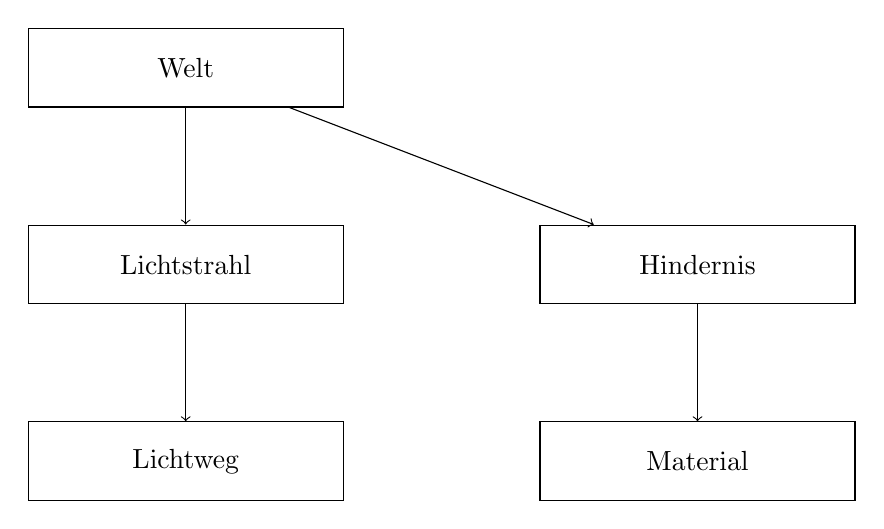
\begin{tikzpicture}[node distance=2.5cm, every node/.style={fill=white, draw=black}, align=center, minimum width=4cm, minimum height=1cm, text centered]
        \node(world)[rectangle]{Welt};
        \node(ray)[rectangle, below of=world]{Lichtstrahl};
        \node(line)[rectangle, below of=ray]{Lichtweg};
        \node(obstacle)[rectangle, right of=ray, xshift=4cm]{Hindernis};
        \node(material)[rectangle, below of=obstacle]{Material};

        \draw[->] (world) -- (ray);
        \draw[->] (world) -- (obstacle);
        \draw[->] (ray) -- (line);
        \draw[->] (obstacle) -- (material);
    \end{tikzpicture}
    \caption{Schematischer Aufbau der Simulation \\ Quelle: Eigene Darstellung}
    \label{m1}
\end{figure}

\section{Welt}
Die Welt \code{World} ist der Grundstein für die Simulation. 
Zu diesem virtuellen zweidimensionalen Raum können sämtliche Entitäten hinzugefügt werden. 
Hier werden diese verwaltet, verarbeitet und zur Visualisierung ausgegeben. 

\section{Lichtstrahl}
In der geometrischen Optik geht man bei einem Lichtstrahl \code{Ray} 
von einem Strahl aus, der sich von einem Ursprung $ A $  
geradlinig in eine Richtung mit dem Winkel 
$ \alpha $ ausbreitet. \parencite[vgl.][S. 1041]{tipler2015physik} mathematisch 
wird dieser als Halbgerade angesehen $ \overrightarrow{AB} $. 
In der Simulation ist es sinnvoll lediglich den Startpunkt als Ortsvektor $ \vec{O} $ \code{origin} innerhalb der Welt
und den Winkel \code{angle}, in den der Strahl ausgeht direkt zu speichern. 

\section{Lichtweg}
Es muss davon ausgegangen werden, dass ein Lichtstrahl in der 
die Kollision mit anderen Objekten seine Richtung verändert. 
Ab einer Richtungsänderung wird der bisherige Lichtstrahl als Lichtweg \code{Line} 
gespeichert, um in später zu visualisieren.
Hierbei besteht ein Lichtstrahl aus den Ortsvektoren $ \vec{O} $ \code{origin} dem 
Ursprung des Lichtstrahls und $ \vec{E} $ \code{end} dem Punkt der Kollision.

\section{Hindernis}
Bei allen Entitäten in der Welt, die nicht Strahl oder Lichtweg sind, 
handelt es sich um Hindernisse. 
Dieser definieren sich durch ihre geometrische Form und Position in der Welt 
und können von Lichtstrahlen getroffen werden.
Es sind verschiedene Variationen möglich. Jedes Hindernis \code{Obstacle} 
hat jedoch einen Startpunkt als Ortsvektor $ \vec{A} $ \code{start} in der Welt. 
Und ein Material \code{material} (vgl. \ref{material}). 
Folgende Typen wurden für diese Arbeit ausgewählt, eine Erweiterung ist jedoch möglich: 

\subsection{Kreis}
Der Kreis \code{type: 'cirlce'} hat eine zusätzliche Angabe über den Radius $ r $ \code{radius}.

\subsection{Linie}
Neben einen Anfangspunkt hat die Linie \code{type: 'line'} auch einen Ortsvektor $ \vec{B} $ als Endpunkt. 

\subsection{Kurve}
Zusätzlich kann ein Hindernis auch eine Kurve \code{type: 'curve'} sein. 
Das ermöglicht die Konstruktion verschiedener besonderer Reflektoren (z. B. Parabolischer Reflektor).
Für den Verlauf der Kurve besitzt dieser Hindernis-Typ eine Funktion $ f $. 
Um eine Kurve beliebig in der Welt zu positionieren, kann ihr zusätzlich eine Winkel $ \gamma $ \code{rotation} übergeben werden, 
der alle Punkte auf Kurve relative zum Ursprung rotiert. \\
Im Umfang dieser Arbeit wird bewusst auf eine vollständige und genaue Darstellung eines Graphen verzichtet. 
Daher werden nur Punkte in einem Interval $ [-40, 40] $ im Abstand von einer übergebene Skalierung $ k $ \code{scale} errechnet, 
als Linien verbunden und als diese Fortlaufend verarbeitet. 
Diese Annäherung ist ausreichend, während gleichzeitig der Umfang stark reduziert wird.


\section{Material}
\label{material}
Die Existenz eines Materials \code{Material} in der Welt besteht nur in der Verknüpfung zu einem Hindernis. 
Ein Material ist für die Verarbeitung eines einfallenden, mit dem Hindernis kollidierenden, Lichtstrahls verantwortlich 
und kann eine beliebig Anzahl an neuen Lichtstrahlen zurückgeben. \\ 
In dieser Arbeit wird nur die Reflexion bei dem Material Spiegel \code{mirror} behandelt. 
Eine Trennung von Material und Hindernis ermöglicht jedoch eine einfache Erweiterung.
Dabei können trotz Veränderung der strahlenoptischer Funktion, die geometrischen Eigenschaften beibehalten werden.
So könnte beispielsweise ein Kreis einerseits als Spiegel die Lichtstrahlen reflektieren 
und anderseits als Glas die Lichtstrahlen brechen. Ohne das dafür die Veränderung des Hindernisses von Nöten wäre.


\chapter{Technische Voraussetzungen}
Um die Zugänglichkeit der Simulation zu erhöhen, wird diese als Web-App programmiert. 
Dazu wird die Programmiersprache TypeScript benutzt und die Applikation wird mit dem Framework „SvelteKit“\footnote{https://kit.svelte.dev} kompiliert.
Zur Visualisierung wird die Library „Pts“\footnote{https://ptsjs.org} verwendet. Diese ermöglicht eine einfache Verwendung der Canvas-API. 
Zusätzlich werden aber auch einige mathematisch Hilfsfunktionen von dieser Library verwendet.

Der gesamte Quellcode für die Simulation ist auf GitHub aufzufinden\footnote{https://github.com/b3ngg/ray-optics-simulation}. 
Im Folgenden werden nur kleine, unvollständige Ausschnitte aus dem Code eingebunden. 
Die fertige Web-App ist ebenfalls als Website aufrufbar\footnote{https://optics.b3n.gg}.


\chapter{Simulationsprozess}
Im Folgenden wird nun der Ablauf der Simulation vom erstellen der Szene bis hin zum Visualisieren des Resultats beschrieben.

\section{Erzeugen der Welt}
Zunächst muss für die Simulation eine Umgebung errichtet werden. Dazu wird eine Welt erstellt.
Zu dieser werden in dieser Szene ein von links oben (man beachte, dass das Koordinatensystem den 
Ursprung links oben hat und die y-Achse umgekehrt zum normalen Koordinatensystem ist) beginnender und diagonal nach rechts 
unten strahlender Lichtstrahl hinzugefügt. \\
Zudem wird auch ein Hindernis in der Form einer vertikalen Linie in der Mitte der Szene hinzugefügt. 
Diese hat das Material Spiegel \code{mirror}. \\ 
Nun wird mit \texttt{world.update()} die Simulation aktualisiert und die Lichtwege berechnet. Dieser werden zum Schluss visualisiert.

Bei den Objekt \texttt{space} handelt es sich um ein von Pts bereitgestellte und zur Visualisierung benötigte Objekt. 
Die Klasse \texttt{Pt} ist ebenfalls Teil von Pts und wird zur Vektormathematik verwendet.
\newpage

\begin{verbnobox}[\scriptsize\mbox{}]
/**
 * Simple reflection of a ray on a vertical line
 */
export const lineReflection: Scene = (space) => {
    const form = space.getForm();
    const world = createWorld();

    world.addSource('ray', createRay(new Pt(), Math.PI * 2.25));
    world.addObstacle(
        'line',
        createLine(new Pt(800, 0), { end: new Pt(800, 5000), material: mirror })
    );

    world.update();
    space.add(() => {
        world.draw(form);
    });

    space.playOnce();
};
\end{verbnobox}

\section{Berechnung des Lichtwegs}
Bei der Berechnung eines Lichtwegs startet die Simulation nur mit einem Ausgangs-Lichtstrahl.
Zunächst muss die erste Überschneidung des Strahls mit einem Hindernis bestimmt werden. 
Für die Bestimmung des Schnittpunktes werden die üblichen Verfahren der Euklidischen Geometrie benutzt. 
Die Funktionen dafür werden von Pts bereitgestellt und sollen hier nicht weiter vertieft werden. \\ 
Der Weg von $ \vec{O} $ des Lichtstrahls bis zum Schnittpunkt $ \vec{E} $ wird dann als Lichtweg gespeichert und später visualisiert.
Aus der Kollision mit dem Hindernis und dem entsprechenden Material können dann weitere Lichtstrahlen resultieren. 
Diese Lichtstrahlen durchlaufen den gleichen Prozess wie der erste Lichtstrahl. 
Daher wird die Funktion als rekursive Funktion verwendet und mit den jeweils neuen Lichtstrahlen erneut aufgerufen.


\begin{verbnobox}[\scriptsize\mbox{}]
const calculateTraceLines = (
    currentRay: Ray,
    lines: PtIterable[],
    depth: number
): PtIterable[] => {
    // Prevent infinite reflections
    if (depth >= MAX_TRACE_DEPTH) return lines;

    // Get all collisions
    const allCollisions = getAllCollisions(currentRay, obstacles);

    // Get best collision
    const collision = getFirstCollision(allCollisions, currentRay.origin);

    // Return the lines and the current ray if not collision is found
    if (!collision) return [...lines, rayToPts(currentRay)];

    const { intersection, collider, obstacle } = collision;

    // Get new rays resulting of the collision
    const newRays = obstacle.material.handleCollision(intersection, collider, currentRay, obstacle);

    // Trace new rays
    return newRays
        .map((ray) => {
            return calculateTraceLines(ray, [...lines, [currentRay.origin, intersection]], depth + 1);
        })
        .flat();
    };
\end{verbnobox}

\section{Berechnung der Reflexion}
Bei dem Material des Spiegels wird für jeden eintreffenden Lichtstrahl ein neuer Lichtstrahl mit verändertem Winkel zurückgegeben. 
Hierbei gilt das Fermat’sche-Prinzip \parencite[vgl.][S. 20]{hering2017optik}.


\subsection*{An einer Linie}
Das Hindernis der Linie kann als eine ebene Grenzfläche angenommen werden. 
Demnach ist der Betrag des Einfallswinkel $ \varepsilon $ relative zum Lot der Grenzfläche gleich mit dem Reflexionswinkel $ \varepsilon_r $. 

\begin{equation}
    -\varepsilon = \varepsilon_r
\end{equation}
\begin{figure}
    \centering
    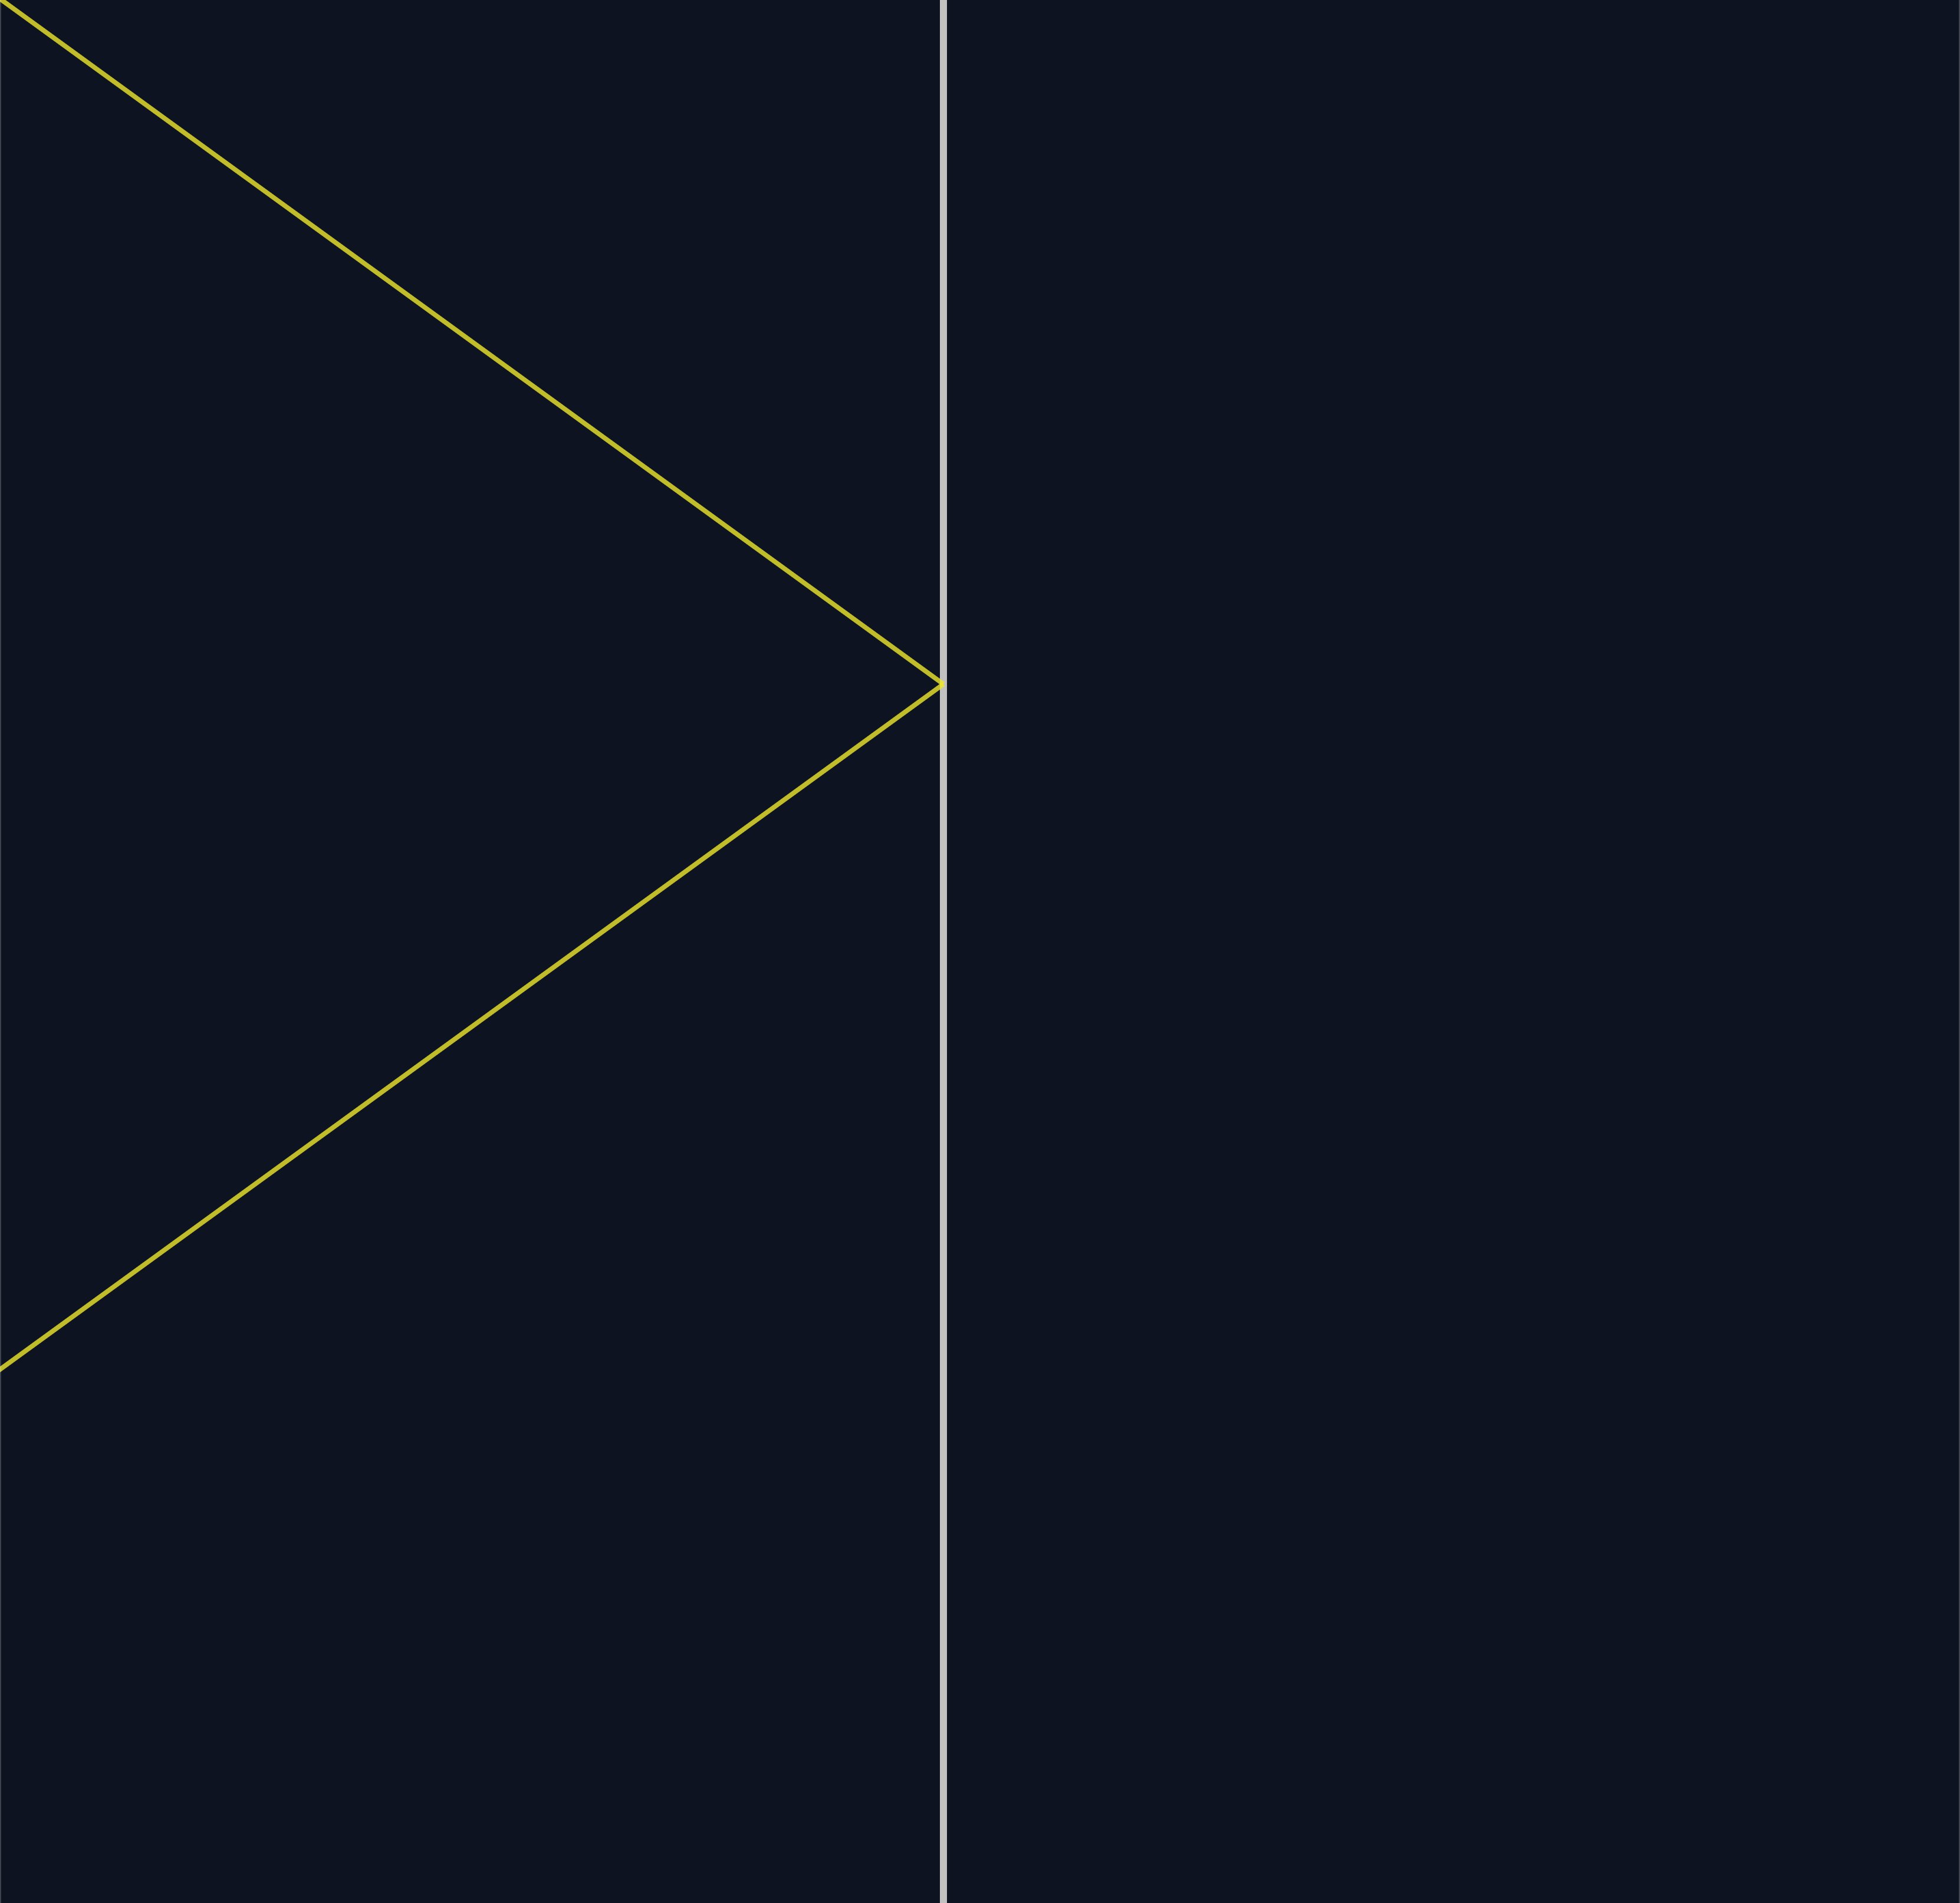
\includegraphics[width=0.5\textwidth]{line-reflection.png}

    \caption{Reflexion eines Lichtstrahls an einer Linie in der Simulation  \\ Quelle: Eigene Darstellung}

\end{figure}
Es gilt daher zunächst den Lot der Linie zu berechnen. Das Lot ist orthogonal zur Linie. 
Es kann berechnet werden, indem der Vektor der Linie in zwei Teile zerlegt wird. \parencite[vgl.][S. 1]{greve2006raytracing}

\begin{verbnobox}[\scriptsize\mbox{}]
/** Calculate the normal point of a line */
const getLineNormal = (line: PtIterable): Readonly<Pt> => {
    const normalAngle = line[0].$subtract(line[1]).angle() + Math.PI / 2;
    return new Pt(0, 1).toAngle(normalAngle).$unit();
};
\end{verbnobox}
Mit dem Lot $ \vec{N} $ und dem Einfallsvektor $ \vec{E} $ lässt sich nun der Reflexionsvektor $ \vec{R} $ berechnen. \parencite[vgl.][Kapitel 10]{cross2013raytracing}
\begin{equation}
    \label{reflexion}
    \vec{R} = \vec{E} - (\vec{E} \cdot \vec{N})\vec{N}
\end{equation}
Gleichung \ref{reflexion} implementiert, sieht wie folgt aus und gibt den neuen reflektierten Lichtstrahl zurück. 
Die Klasse \texttt{Vec} ist von Pts bereitgestellt und beinhaltet Operationen der Vektormathematik.

\begin{verbnobox}[\scriptsize\mbox{}]
/** Calculate the reflected ray of an incoming ray with the angle d to a line on a point */
const getReflectedRayOnLine = (
    incidentRay: Ray,
    line: PtIterable,
    collisionPoint: Pt
): Readonly<Ray> => {
    const d = new Pt(1, 0).toAngle(incidentRay.angle);
    const lineNormal = getLineNormal(line);

    const perpendicular = 2 * Vec.dot(d, lineNormal);
    const reflection = Vec.subtract(d, Vec.multiply(lineNormal, perpendicular));
    const r = new Pt(reflection);

    return createRay(collisionPoint, r.angle());
};
\end{verbnobox}

\subsection*{An einem Kreis}
Ein Kreis kann als Konvexspiegel mit dem Mittelpunkt $ M $ und dem Brennpunkt $ F $ angesehen werden. \parencite[vgl.][S. 362]{kuchling2004taschenbuch}
Wobei bei einem Kreis folgendes gilt: 
\begin{equation}
    \label{mequalf}
    M = F
\end{equation}
\ref{mequalf} nach ergibt sich für den Reflexionsvektor $ \vec{R} $ mit dem Mittelpunkt $ \vec{M} $ und dem Schnittpunkt $ \vec{E} $ folgende Gleichung:
\begin{equation}
    \label{circlereflexion}
    \vec{R} = \vec{E} - \vec{M}
\end{equation}
Um Gleichung \ref{circlereflexion} zu implementiert genügt lediglich folgender Quellcode:

\begin{verbnobox}[\scriptsize\mbox{}]
/** Calculates the reflected ray of an incoming ray on a circle */
const getReflectedRayOnCircle = (collisionPoint: Pt, circleCenter: Pt): Readonly<Ray> => {
    const perpendicularAngle = collisionPoint.$subtract(circleCenter).angle();
    return createRay(collisionPoint, perpendicularAngle);
};
\end{verbnobox}

\begin{figure}
    \centering
    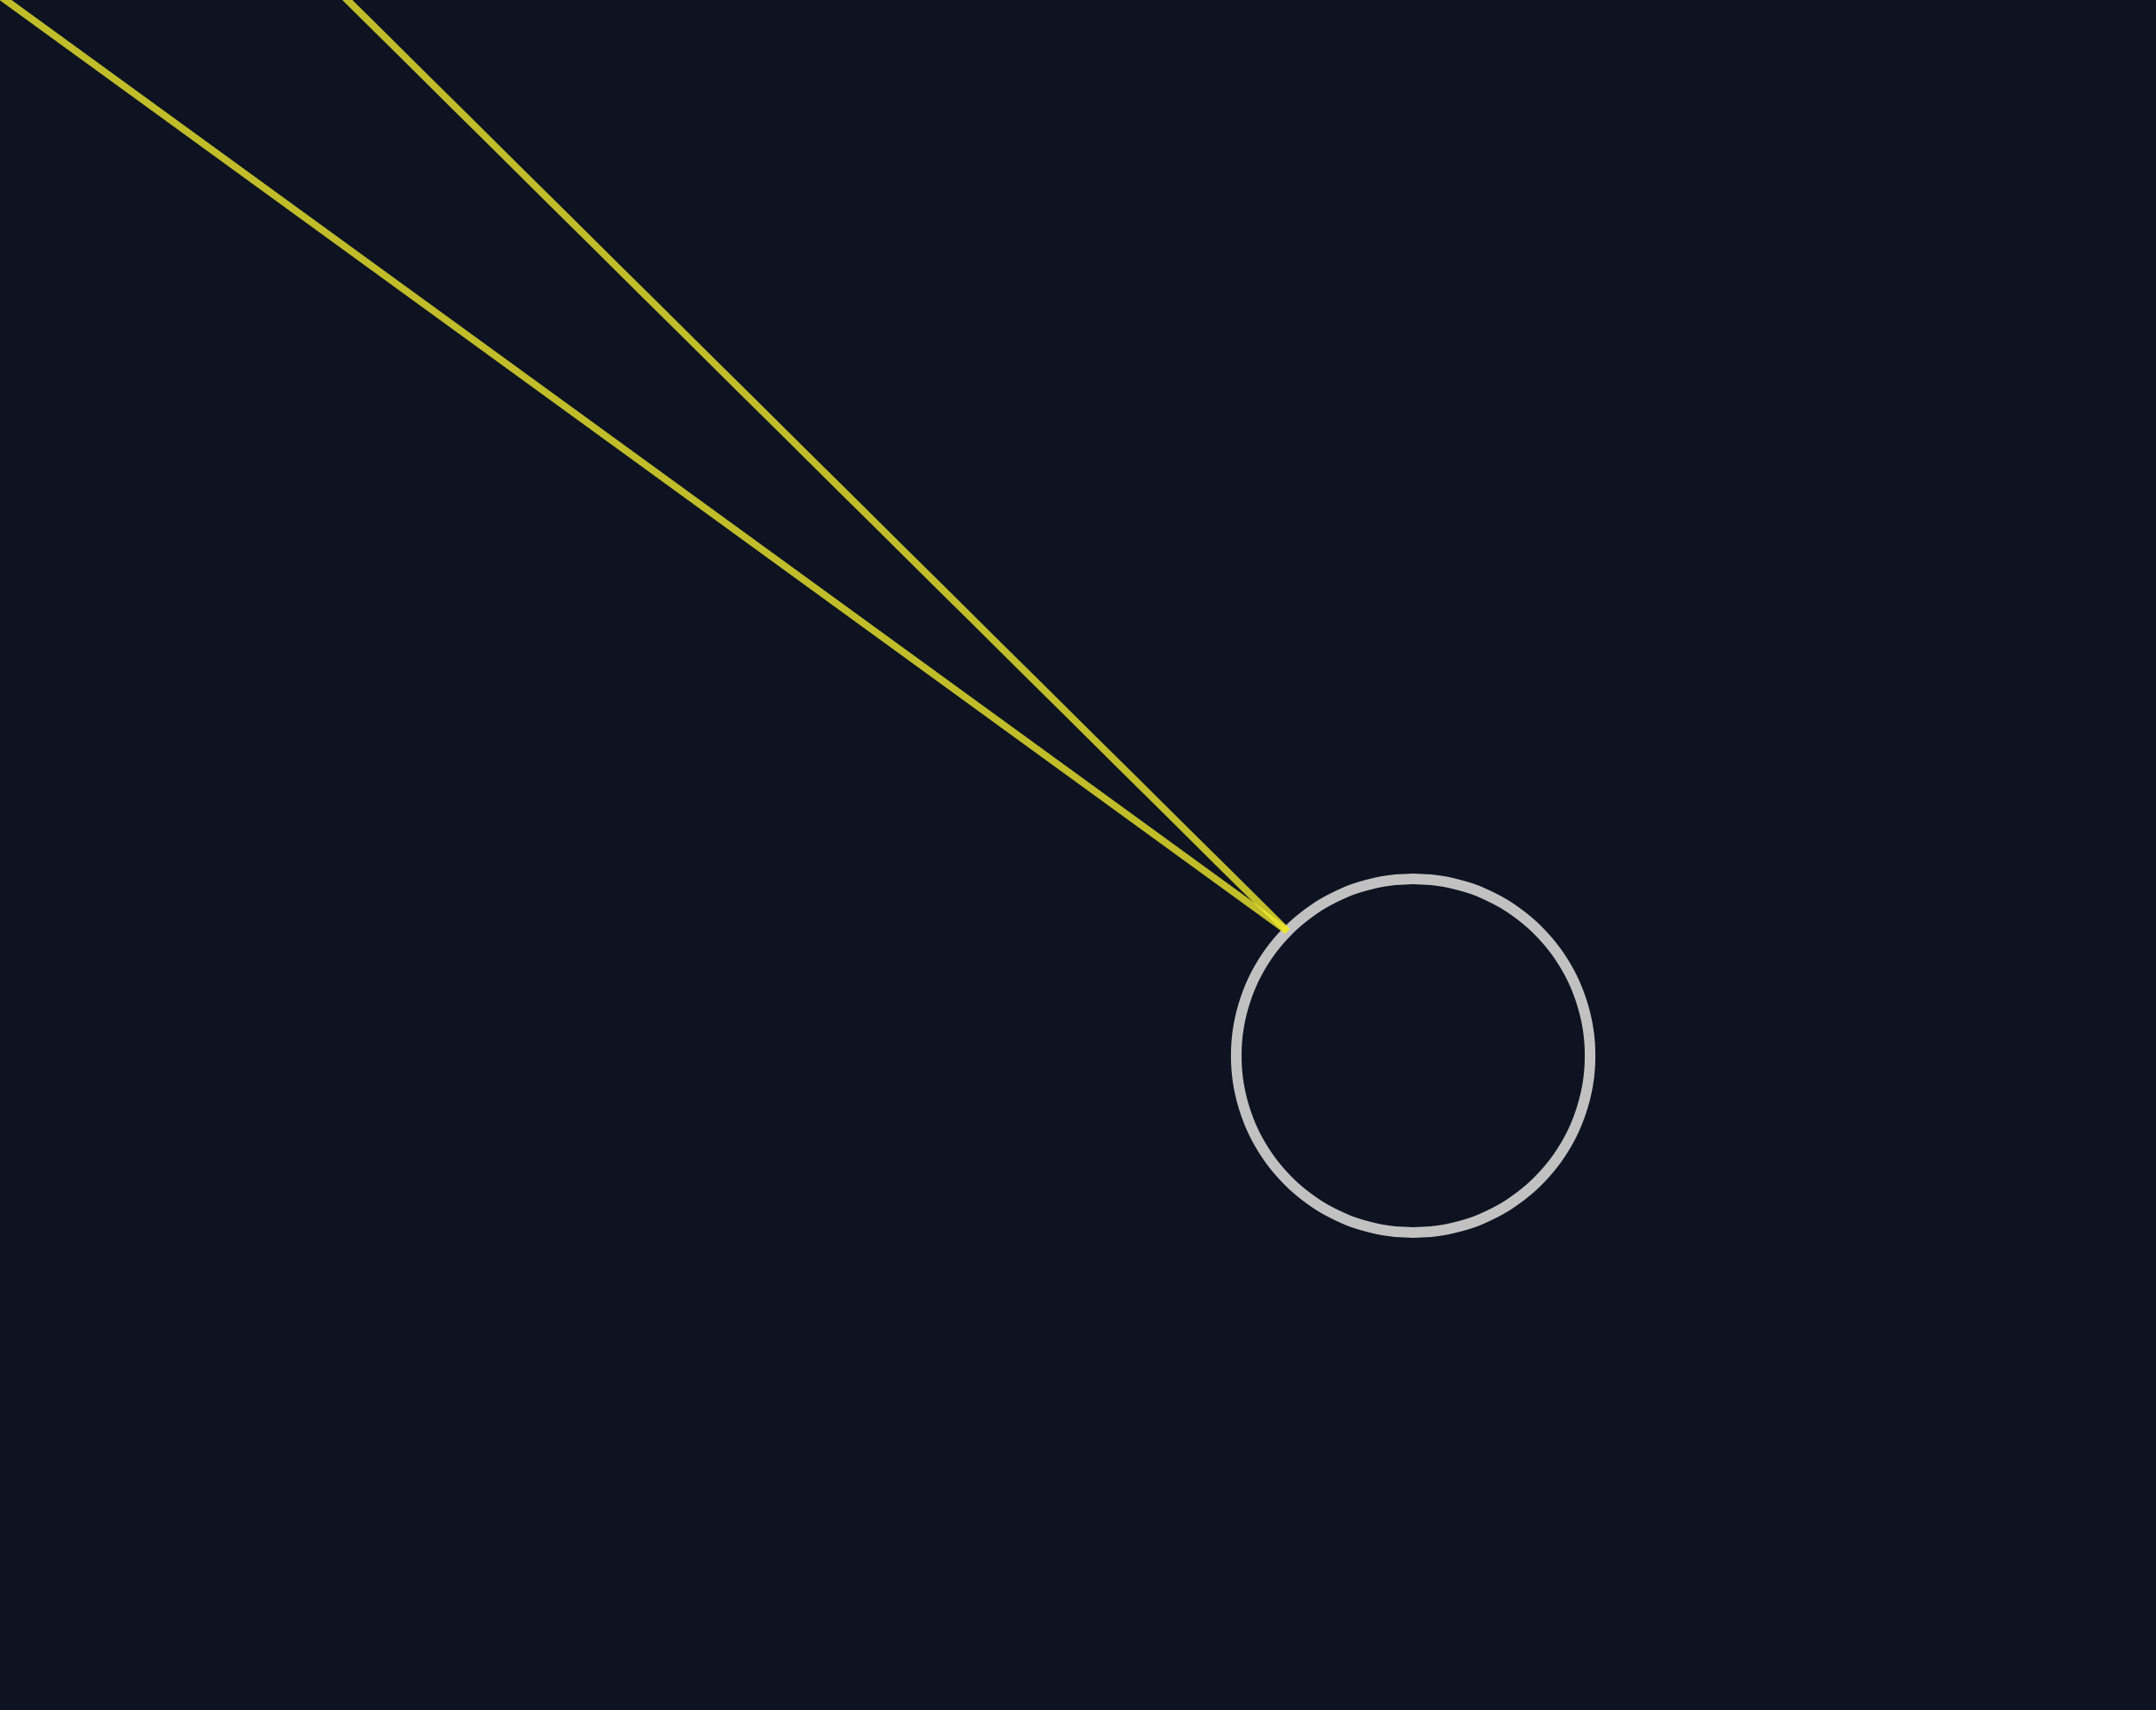
\includegraphics[width=0.5\textwidth]{circle-reflection.png}

    \caption{Reflexion eines Lichtstrahls an einem Kreis in der Simulation  \\ Quelle: Eigene Darstellung}

\end{figure}

\chapter*{Zusatz: Komplexe Umgebungen}
Im Folgenden sollen komplexere Umgebungen und deren Resultat in der Simulation demonstriert werden. 
Weitere interaktive Beispiele sind online\footnote{https://optics.b3n.gg} aufzufinden.
\newpage
\subsection*{Parabolischer Reflektor}
Bei einer parabolischen Reflektor handelt es sich um einen Konkavspiegel. \parencite[vgl.][S. 362]{kuchling2004taschenbuch}.
Senkrecht einfallende Strahlen werden hierbei zu einem Brennpunkt reflektiert. 

\begin{verbnobox}[\scriptsize\mbox{}]
/**
* Reflections of multiple rays on a parabolic reflector
*/
export const parabolic: Scene = (space) => {
    const form = space.getForm();
    const world = createWorld();

    for (let i = 0; i < 10; i++) {
        world.addSource('ray' + i, createRay(new Pt(500 + 40 * i, 0), Math.PI * 2.5));
    }

    world.addObstacle(
        'reflector',
        createCurve(new Pt(480 + 5 * 40, 500), { f: (x) => (x / 10) ** 2, scale: 6, material: mirror })
    );

    world.update();
    space.add(() => {
        world.draw(form);
    });

    space.playOnce();
};
\end{verbnobox}

\begin{figure}
    \centering
    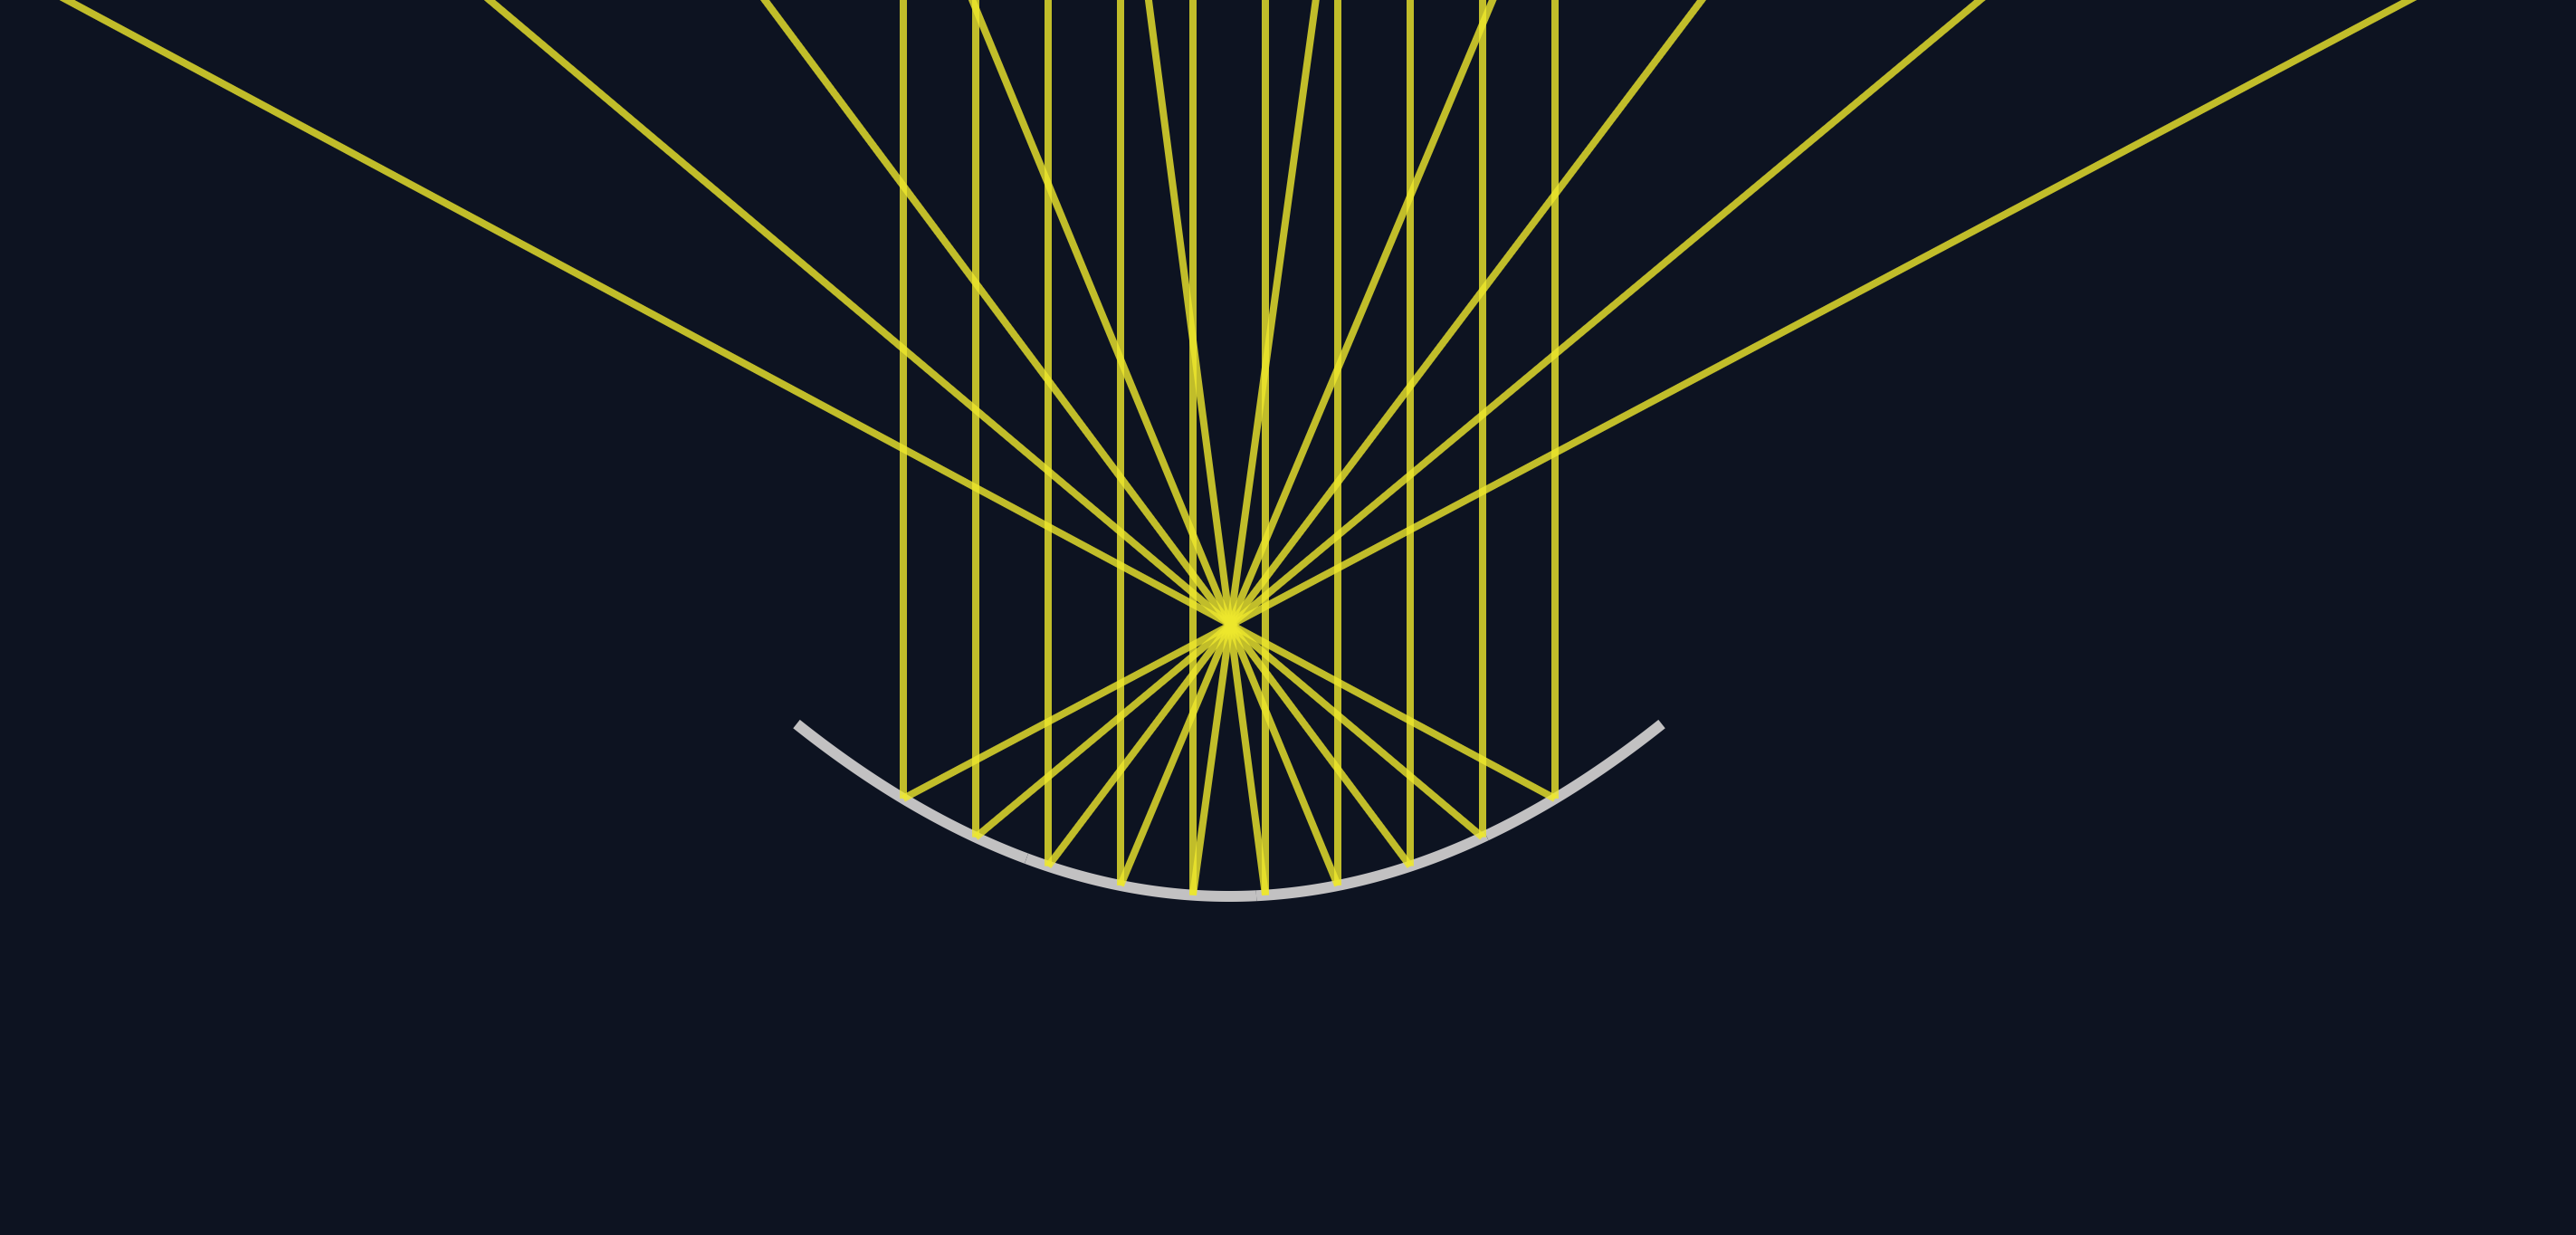
\includegraphics[width=\textwidth]{parabolic.png}

    \caption{Reflexion mehrere Lichtstrahlen an einem parabolischen Reflektor  \\ Quelle: Eigene Darstellung}

\end{figure}
\newpage

\subsection*{Reflexion an Kreisen}
Bei einer großen Anzahl an Kreisen entwickeln sich sehr schnell viele Reflexionen. Eine Art Stress-Test für die Simulation.
\begin{verbnobox}[\scriptsize\mbox{}]
export const circleChaos: Scene = (space) => {
    const form = space.getForm();
    const world = createWorld();
    space.add({
        start: (bound) => {
            const pts = Create.distributeRandom(bound, 30);
            pts.forEach((pt, i) => {
                world.addObstacle('circle' + i, createCircle(pt, { material: mirror, radius: 60 }));
            });

            world.addSource('dynamic-ray', createRay(space.center, Const.pi));
        }
    });
    space.playOnce();
};
\end{verbnobox}

\begin{figure}
    \centering
    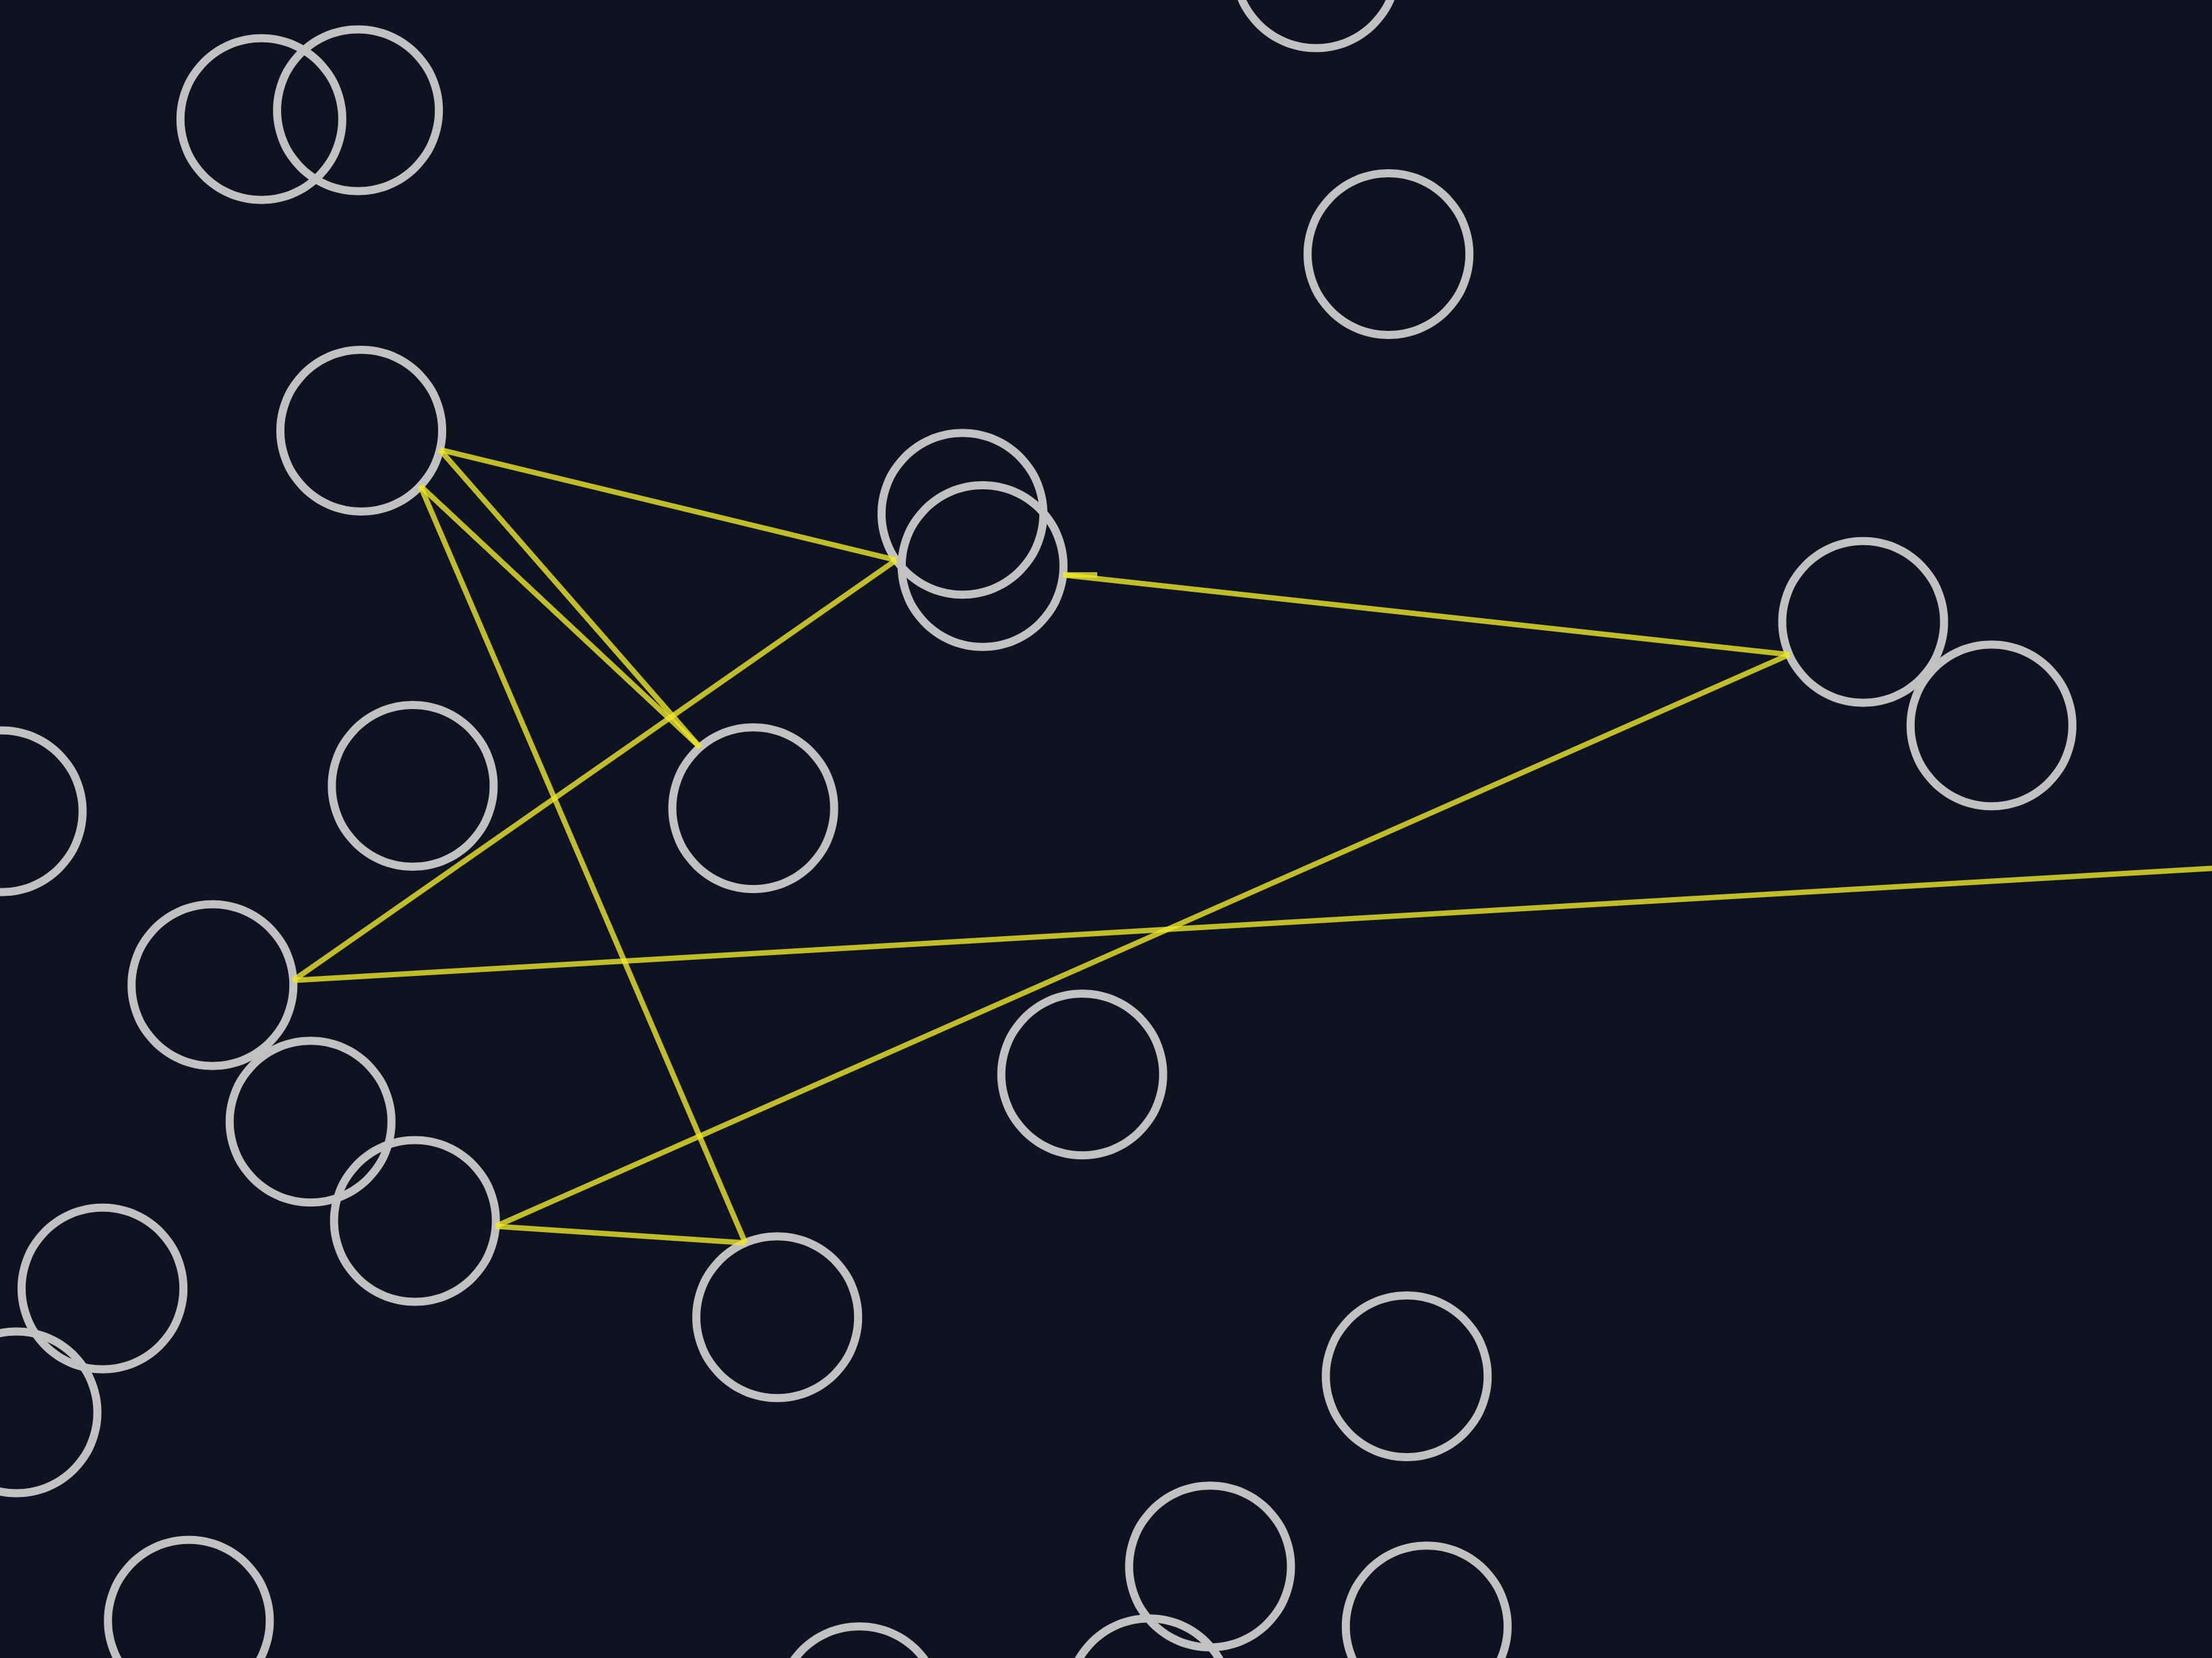
\includegraphics[width=\textwidth]{chaos.png}

    \caption{Reflexion eines Lichtstrahls an vielen Kreisen \\ Quelle: Eigene Darstellung}

\end{figure}